\begin{pastexam}[label={px:gk3-105-ds-02}]{高考三級資訊處理 105 年 第二題}
（申論；20 分）

\begin{itemize}[leftmargin=2.2em]
\item[㈠] 請將下列值 2, 1, 4, 5, 9, 3, 6, 7 依序插入原來為空的紅黑樹（red-black tree），請寫出結果。作答時，
請標示節點如下：例如節點 2B 表示其值為 2 的黑（Black）節點，又如節點 5R 表示其值為 5 的紅（Red）節點。（10 分）
\item[㈡] 請畫出與上面㈠小題相對應的 2-3-4 樹（2-3-4 tree）。（10 分）
\end{itemize}
\end{pastexam}

\begin{pastsoln}
答案：㈠ 根 $2$B；$2$ 的左子 $1$B、右子 $5$R；$5$ 的左子 $4$B、右子 $7$B；$4$ 的左子 $3$R；$7$ 的左子
$6$R、右子 $9$R。 ㈡ 根 $[2\ 5]$，三個子節點 $[1]$、$[3\ 4]$、$[6\ 7\ 9]$。

\textbf{㈠} 用資結書第~10.3~節的插入（虛擬碼~10.6）：新節點先照二元搜尋樹插入、塗紅；若父節點也是
紅的，看叔叔 $u$ 的顏色修正——情況 1（$u$ 紅）：父、叔改黑，祖父改紅，再從祖父往上檢查；情況 2
（$u$ 黑，$z$ 在內側）：對父節點旋轉，變成情況 3；情況 3（$u$ 黑，$z$ 在外側）：父改黑、祖父改紅，
對祖父旋轉。 最後根塗黑。 空指標當成黑色。
\begin{itemize}
\item $2$：成為根，塗黑。 $2$B。
\item $1$：$2$ 的左子，父 $2$ 是黑的，不用修正。
\item $4$：$2$ 的右子，父黑，不用修正。 圖 (a)。
\item $5$：$4$ 的右子。 父 $4$ 紅、叔叔 $1$ 紅，情況 1：$4$、$1$ 改黑，$2$ 改紅；$2$ 是根，塗回黑。
圖 (b)，黑高度加一。
\item $9$：$5$ 的右子。 父 $5$ 紅、叔叔（$4$ 的左子）是空的、算黑；$9$ 是右子的右子，在外側，情況 3：
$5$ 改黑、$4$ 改紅，對 $4$ 左旋。 圖 (c)。
\item $3$：$2 \to 5 \to 4$，成為 $4$ 的左子。 父 $4$ 紅、叔叔 $9$ 紅，情況 1：$4$、$9$ 改黑，$5$ 改紅；
往上看 $5$，它的父 $2$ 是黑的，停止。
\item $6$：$2 \to 5 \to 9$，成為 $9$ 的左子，父 $9$ 黑，不用修正。 圖 (d)。
\item $7$：$2 \to 5 \to 9 \to 6$，成為 $6$ 的右子。 父 $6$ 紅、叔叔（$9$ 的右子）空、算黑；$7$ 是左子的
右子，在內側，情況 2：對 $6$ 左旋，$7$ 上來、$6$ 成為 $7$ 的左子；接著情況 3：$7$ 改黑、$9$ 改紅，
對 $9$ 右旋。 圖 (e)，就是最後結果。
\end{itemize}
\begin{center}
\begin{tikzpicture}[every node/.style={ellipse,draw,minimum height=6mm,minimum width=8mm,inner sep=1pt,font=\small},
  bk/.style={fill=black,text=white}, rd/.style={draw=red!70!black,very thick,fill=red!12},
  lab/.style={draw=none,fill=none,font=\small},
  level distance=9mm, level 1/.style={sibling distance=14mm}, level 2/.style={sibling distance=10mm}]
\node[bk] {2B} child {node[rd] {1R}} child {node[rd] {4R}};
\node[lab] at (0,-2.9) {(a) 插入 2、1、4};
\begin{scope}[xshift=32mm]
\node[bk] {2B} child {node[bk] {1B}} child {node[bk] {4B} child[missing] child {node[rd] {5R}}};
\node[lab] at (0,-2.9) {(b) 插入 5};
\end{scope}
\begin{scope}[xshift=66mm]
\node[bk] {2B} child {node[bk] {1B}} child {node[bk] {5B} child {node[rd] {4R}} child {node[rd] {9R}}};
\node[lab] at (0,-2.9) {(c) 插入 9};
\end{scope}
\end{tikzpicture}

\medskip
\begin{tikzpicture}[every node/.style={ellipse,draw,minimum height=6mm,minimum width=8mm,inner sep=1pt,font=\small},
  bk/.style={fill=black,text=white}, rd/.style={draw=red!70!black,very thick,fill=red!12},
  lab/.style={draw=none,fill=none,font=\small},
  level distance=9mm, level 1/.style={sibling distance=20mm}, level 2/.style={sibling distance=14mm},
  level 3/.style={sibling distance=9mm}]
\node[bk] {2B} child {node[bk] {1B}}
  child {node[rd] {5R} child {node[bk] {4B} child {node[rd] {3R}} child[missing]}
                       child {node[bk] {9B} child {node[rd] {6R}} child[missing]}};
\node[lab] at (0.5,-3.6) {(d) 插入 3、6};
\begin{scope}[xshift=60mm]
\node[bk] {2B} child {node[bk] {1B}}
  child {node[rd] {5R} child {node[bk] {4B} child {node[rd] {3R}} child[missing]}
                       child {node[bk] {7B} child {node[rd] {6R}} child {node[rd] {9R}}}};
\node[lab] at (0.5,-3.6) {(e) 插入 7，最後結果};
\end{scope}
\end{tikzpicture}
\end{center}
（黑底白字是黑節點，粗框淺底是紅節點，節點上也照題目寫了 B、R。）

檢查性質：根 $2$ 是黑的；紅節點 $5, 3, 6, 9$ 的子節點都是黑的（或空）；從根到每個空指標經過的黑節點
數（含根、不含空指標）都是 $2$，例如 $2 \to 1$、$2 \to 5 \to 4 \to 3$、$2 \to 5 \to 7 \to 9$。 中序是
$1, 2, 3, 4, 5, 6, 7, 9$。

\textbf{㈡} 把每個黑節點和它的紅色子節點合成一個 2-3-4 樹的節點（資結書第~10.4~節、第~11.1~節）：
\begin{itemize}
\item $2$B 和紅子 $5$R 合成 $[2\ 5]$（3-節點）。
\item $1$B 沒有紅子，成為 $[1]$。
\item $4$B 和紅子 $3$R 合成 $[3\ 4]$。
\item $7$B 和紅子 $6$R、$9$R 合成 $[6\ 7\ 9]$（4-節點）。
\end{itemize}
\begin{center}
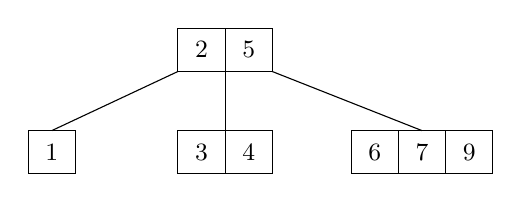
\begin{tikzpicture}[k/.style={draw,minimum width=6mm,minimum height=5.5mm,inner sep=0pt,font=\small}]
\node[k] at (-0.3,0) {2}; \node[k] at (0.3,0) {5};
\node[k] at (-2.2,-1.3) {1};
\node[k] at (-0.3,-1.3) {3}; \node[k] at (0.3,-1.3) {4};
\node[k] at (1.9,-1.3) {6}; \node[k] at (2.5,-1.3) {7}; \node[k] at (3.1,-1.3) {9};
\draw (-0.6,-0.275) -- (-2.2,-1.025);
\draw (0,-0.275) -- (0,-1.025);
\draw (0.6,-0.275) -- (2.5,-1.025);
\end{tikzpicture}
\end{center}
三個葉子都在同一層，根的兩個鍵把子樹分成「小於 $2$」「$2$ 和 $5$ 之間」「大於 $5$」三段，是合法的
2-3-4 樹。 黑高度 $2$ 正好等於 2-3-4 樹的層數。

另一種讀法是「把同樣的數直接插入空的 2-3-4 樹」。 用資結書虛擬碼~11.1 由上而下的插入：$2, 1, 4$
得 $[1\ 2\ 4]$；插入 $5$ 前根是 4-節點，先分裂成 $[2]$ 和 $[1]$、$[4]$，$5$ 放進 $[4\ 5]$；$9$ 放進
$[4\ 5\ 9]$；插入 $3$ 時往右走遇到 4-節點 $[4\ 5\ 9]$，先分裂，$5$ 上到根成 $[2\ 5]$，$3$ 放進 $[3\ 4]$；
$6$、$7$ 放進 $[6\ 9]$、$[6\ 7\ 9]$。 結果和上圖完全一樣，兩種讀法的答案相同。
\end{pastsoln}
